% VLDB template version of 2020-03-05 enhances the ACM template, version 1.7.0:
% https://www.acm.org/publications/proceedings-template
% The ACM Latex guide provides further information about the ACM template

\documentclass[sigconf, nonacm]{acmart}

\usepackage{lipsum}
\usepackage{hyperref} % Hacer referencias bknes
\usepackage{comment}
\usepackage[indent]{parskip} % Para hacer saltos de linea automático
\setlength{\parskip}{0.5\baselineskip minus2pt} % Aquí se modifica el salto de linea
\usepackage{graphicx}
\usepackage{caption}
\usepackage{subcaption}
\usepackage[caption=false]{subfig}

%% The following content must be adapted for the final version
% paper-specific
\newcommand\vldbdoi{XX.XX/XXX.XX}
\newcommand\vldbpages{XXX-XXX}
% issue-specific
\newcommand\vldbvolume{14}
\newcommand\vldbissue{1}
\newcommand\vldbyear{2020}
% should be fine as it is
\newcommand\vldbauthors{\authors}
\newcommand\vldbtitle{\shorttitle} 
% leave empty if no availability url should be set
\newcommand\vldbavailabilityurl{http://vldb.org/pvldb/format_vol14.html}

\begin{document}
\title{Landslide Early-Warning from Satellite Data}
\subtitle{Research Paper Final Submission \\
Universidad de Chile, Santiago, Chile} 

%% ################################################
%% Pongan sus contactos aqui abajo
%% ###############################################

%%
%% The "author" command and its associated commands are used to define the authors and their affiliations.
\author{José Díaz}
\affiliation{}
\email{jose.diaz.v@ug.uchile.cl}

\author{Fabián Lema}
\affiliation{}
\email{fabian.lema@ug.uchile.cl}

\author{Francisco Muñoz}
\affiliation{}
\email{femunoz@dim.uchile.cl}

\author{Kevin Pinochet}
\affiliation{}
\email{kevin.pinochet@ug.uchile.cl}

\author{Tomás Rojas}
\affiliation{}
\email{tomas.rojas.c@ug.uchile.cl}

\author{Victor Faraggi}
\affiliation{}
\email{victor.faraggi@ug.uchile.cl}

%%
%% The abstract is a short summary of the work to be presented in the
%% article.
\begin{abstract}
% Around the world and though out humman history, landslides have been a risk to both humman life and infrastructure. Even so, since the second half of the last century, the effects of climate change have changed erosion, precipitation, forestation, and the soil type. All of them important factors that can increase the frequency and severity of landslides.  This document aims to present the team research question and work plan for the competition ProjectX 2020. 
% For this purpose, interviews where done to field experts, previous research was study and possible usefully data was gathered.

%hola
% 
%mi abstrak : 
Landslides are a major hazard to human life and society's infrastructure. Due to climate change's effect on precipitation, temperature and many other variables involved in the landslide process, a rise in both the severity and occurrence of these events are expected. In the context of ProjectX 2020 research competition, this work will attempt to use machine learning methods to improve current early warning systems from a risk based perspective and taking into account weather variability. %This document presents our team's interviews with domain experts, our proposal, previous research, the expected data that we will need to take into account and our work plan for the rest of the competition.
To achieve this, the team developed three APIs that can access and process relevant data to the problem from several sources and designed a Convolutional Network with LSTM to detect the occurrences of a landslide. The following steps will be the preparation of the training data, the training of the detection model and the evaluation of hyperparameters.

% achieve this... 
\end{abstract}

\maketitle

%\section{Interviews}

% Regarding the approach we decided to take to define our research question, we chose to tackle a regional or local extreme event. This decision was based on two important points. 
% The first one was due to the previous knowledge we had about the intersection of machine learning and extreme weather event prediction: most of the literature focused on events that affected countries from the northern hemisphere [citation needed]. %existen ejemplos de tormentas, huracanes, incendios, etc., voy a buscar
% The second one was because we wanted to strive our work to be applicable to real world events.

%During a time span of two weeks we met with multiple experts that came from different domains such as Hydrological modelling, Landslide and Forest Fire mitigation. % and Water Floods. 

%Our first meeting was with Pablo Mendoza, PhD at Colorado Boulder and Postdoc at University Corporation for Atmospheric Research (UCAR). He introduced us briefly to hydrological modeling and the state of art about machine learning models applied in hydrology. As this was the first expert we met, he encouraged us to ask ourselves important questions that could define what \textit{we} wanted this project to be. 

%The second expert that we met was Alberto de la Fuente, PhD in Engineering Sciences from Universidad de Chile. He remarked that hydrological models are very closely related to statistical ones. In his experience, he has noticed many research projects give too many importance to the tools used to solve the problem rather than the conceptual ideas behind the models.

%The third expert that we met was Pedro Berrios, a firefighter and Engineer that works at the National Service of Geology and Mining of Chile  (\href{https://www.sernageomin.cl/}{Sernageomin}). He told us briefly the context about landslides, how they predict them and how this affects our country. He remarked to us the importance of having a model that can predict the place of a landslide, and he told us that he could provide us with some datasets if we tried to solve this problem. 


%The fourth meeting we had was with Andrés Weintraub, an expert in Forest Fire mitigation, PhD at UC Berkeley and awarded the Chilean National Science Award. First, he explained his current line of research in forest fires: decision making in order to minimize the risk. The exchange allowed us to gain insight on the current state of forest fire modelling and the current needs that Chile is experiencing in this regard. He also explained some introductory methodologies to perform regional and local risk-based analyses. 


%The final expert we met was Juan Pablo Boisier, researcher at the Chilean Center for Climate and Resiliency (\href{https://www.cr2.cl}{CR2}) and PhD in Climate Science at École Polytechnique. On one side, he advised us against focusing on “early predictions” for drought. 

% On the other side, early warning systems for floods or landslides seemed promising. 

% Regarding to forest fires, he expressed that it can be tackled from multiple angles.

% Then, in the case we wanted to work on it, we would be faced with a difficult choice. 

%He insisted that, in order to define a good research question, we would have to ask ourselves which kind of perspective we want to work on. Ultimately, together, we pondered that adding a human risk based factor to our analysis would be a nice way to take our research closer to decision makers. 


%\subsection{Main Takeaways}

%After the interviews, we thought on the extreme events that were most mentioned: forest fires, floods and landslides. There is work to be done on all of them but we needed to decide what kind of perspective we wanted to give to our work. Also, as machine learning practitioners working on geophysical subjects we would have to define a solid conceptual model and then develop our data driven one. In addition, we identified that using human risk based features would make our work more complete and it would make it more relevant to decision makers. 

%As we reviewed the three main extreme events, we decided that landslides were a promising area to work on. Whereas, for forest fires it was pointed out that it would be more difficult to produce meaningful results in only three months and, for floods, it would be much harder to get our hands on relevant data sources.


%\section{Related Research}


%Several related research on landslide events has been done. 
%On the theoretical side, there have been very good attempts to model the phenomena using numerical simulations. For example, given the occurrence of a landslide, there have been attempts to obtain knowledge about the probability density function of the extension and duration of it previous to the event actually takes place \cite{characteristic_scales}. 
%More probabilistic approaches have been taken into consideration, such as using \emph{Information Value}, \emph{Weights of Evidence} and \emph{Certainty Factor} \cite{predictivelandslide}. There have been more ML related approaches, like SVM based techniques or deep learning's Fully Connected Sparse Autoencoder (FC-SAE) \cite{fcsae}, used in landslide susceptibility modeling \cite{svmlandslide}. There's been also studies of several deep learning approaches applied to deep-seated landslides. \cite{deep_seated_implementations} Has reviewed multiple machine learning based nowcasting strategies applied to the latter, ranging from LSTM to ELM SVM.


%\section{Why is this problem relevant to climate?}

%With the exacerbation of climate change; droughts, precipitations, soil changes and other phenomena have become more extreme while at the same time becoming more unpredictable. \cite{climatechangeimpacts}. 
%This fact is of great relevance considering that intense rainfall events, rapid snow melt, storm waves and deforestation are some of the most important trigger factors of landslides \cite{libro_geologia}.


%In the case of northern and central Andean regions of Chile, several studies \cite{boisier, falvey, garreaud} have shown important changes in climate patterns trends since the last four decades. Particularly, there has been an increase in temperatures of 0,25°C per decade, while it is expected that precipitations will decrease in the next decades, even reaching deficits between 25\% and 50\%. It is expected that these significant changes in the regional climate will affect the frequency and magnitude of landslides.

%The climate crisis we are facing as a planet is not only affecting the environment, but also affecting thousands of millions \cite{landslidesandclimatechange}. In Chile, landslides has affected numerous communities located in Andes's foothills. According to data from SERNAGEOMIN, between 1980 and 2017 there has been at least 214 deaths in the country because events like landslides and debris flows \cite{sernageomin}.

%\section{Research Question}

%One of the important points missing that we noticed is the lack of consideration to the risks related to this phenomena. By risk we understand, as said by Pedro Berrios, ``the danger affecting communities, ranging from material losses to death''. Another factor to take into account is the need of an adaptive model that takes into account future weather data variability. In this context, our main goal is to answer the following: 



%\textit{Taking into account the current weather variability and the risk, as defined above: How can we improve the current early-warning systems with statistical models? moreover: Is it possible to predict the place and time of occurrence of landslides?}


%\section{Why use Machine Learning?}
% En esta sección faltan MUCHAS referencias uwu

%As Pedro told us in his interview, in remote and isolated populations there is not enough resources or money for a complex monitoring system, so availability of real time data for all catchments can be non feasible. However, historical data and real-time weather data is available hence allowing for a ML model that takes of this to be a solution worth of consideration.   

%Moreover, the data at hand uses different types of formats, e.g. gridded weather data or local remote sensing from susceptible slopes. Therefore, techniques that can take advantage of this multiplicity of formats are essential. This is where ensemble learning \cite{ensembles} or other machine learning methods \cite{other_data_fusion} can be of use. 

%Given this, the opportunity to use machine learning seems clear. Due to its ability to find complex or hidden correlations between the data sources, depending of the type of models used. 

%As a side note, as a result from our meeting with Pedro Berrios, we are aware that currently ONEMI's emergency alerts for landslides is based on expert human criteria that analyses each of the available observations. It's not difficult to deduce that the implementation of a machine learning model would improve this repetitive task and thus making experts available to do more relevant work. %


%\section{Type of Research Contribution}

%The contribution would be the implementation of new techniques and ML models to evaluate the real-time risk of a landslide, prioritizing the prevention of human losses. Also, using the datasets and information that is available in Chile and low density regions.  %


% Una definicion del problema, que buscamos hacer, pregunta de investigacion
\section{Introduction}

% Relevancia del estudio
% Qué se ha hecho / Qué hemos hecho (Esto es el background)
% Lo que queremos hacer
% Objetivos

%Porq este problema es relevante, porq tiene q ver con cambio climatico, porq usar ML y trabajos previos
%\subsection{Background}

With the exacerbation of climate change; droughts, precipitation, soil changes and other phenomena have become more extreme while at the same time becoming more unpredictable. \cite{climatechangeimpacts}. 
This fact is of great relevance considering that intense rainfall events, rapid snow melt, storm waves and deforestation are some of the most important trigger factors of landslides \cite{libro_geologia}.


%In the case of northern and central Andean regions of Chile, several studies \cite{boisier, falvey, garreaud} have shown important changes in climate patterns trends since the last four decades. Particularly, there has been an increase in temperatures of 0,25°C per decade, while it is expected that precipitations will decrease in the next decades, even reaching deficits between 25\% and 50\%. It is expected that these significant changes in the regional climate will affect the frequency and magnitude of landslides.

The climate crisis we are facing as a planet is not only affecting the environment, but also affecting thousands of millions of people \cite{landslidesandclimatechange}. Particularly, this crisis has been materialized in an increase of frequency and intensity of catastrophes events like landslides. Sample of the social effect they have had can be seen in the records from the National Service of Geology and Mining of Chile \href{https://www.sernageomin.cl/}{(SERNAGEOMIN)}, according to which numerous communities located in Andes's foothills have been affected by landslides events. In more detail, between 1980 and 2017 there have been at least 214 deaths in this country because of events like landslides and debris flows \cite{sernageomin}. 

In that context, one of the principal motivations and important points missing that is noticed by the team is the lack of consideration to the risks related to this phenomena. The risk will be understood as said by Pedro Berrios, Engineer that works at \href{https://www.sernageomin.cl/}{SERNAGEOMIN}, ``the danger affecting communities, ranging from material losses to death''. Another factor to take into account is the need of an adaptive model that takes into account future weather data variability. Considering this background, the main goal of this project is to answer the following question:


\textit{Taking into account the current weather variability and the risk, as defined above: How can the current early-warning systems be improved through
the use of statistical models? moreover: Is it possible to predict the place and time of occurrence of landslides?}

Therefore, this paper proposes a ML oriented method for early-warning of landslide events using satellite information. This in order to provide, in the future, helpful data to government offices and decision-makers, such as the National Emergency Office of the Ministry of the Interior of Chile\href{https://www.onemi.gov.cl/}{(ONEMI)}, that can contribute them to take informed decisions.

To achieve this, the following objectives are proposed:
\begin{enumerate}
    \item Find and define the datasets that are going to be used.
    \item Extract and preprocess relevant information from the datasets.
    \item Process the datasets and create training data.
    \item Create and implement a first model of landslides prediction.
    \item Obtain preliminary results and define the next steps.
\end{enumerate}


% Parrafo con la estructura del informe (secciones)

\section{Methodology}

For the initial development of an early-warning system four main components are identified: the data description and extraction and the landslide prediction. % and the risk factor.

\subsection{Assumptions}

Two main assumptions were considered in this work: the first one being that landslides events are independent of location and time, this introduces obvious flaws, for instance, a landslide cannot occur in the center of a big city, hence this assumption is erroneous, but we also intend this model to be used in parts where it does make sense trying to know an early prediction. We also considered that the scales, both spatial and temporal are such that no information regarding the processes involved is lost, this is controversial and will be discussed afterwards.


\subsection{Description of Datasets considered in this work} \label{ss:datasets-considered}

%\section{Datasets}


\begin{itemize}
    \item Slope, Land use, Topography, Soil moisture, Precipitation, Snow melting and Deformation. All of this key variables will be taken from satellite observation data offered by Descartes Lab.
    \item \href{https://maps.nccs.nasa.gov/arcgis/apps/webappviewer/index.html?id=824ea5864ec8423fb985b33ee6bc05b7}{NASA Landside Viewer}.
    \item Remote sensing products, like ASTER GDEM, MODIS and Landsat satellites images. These tools can provide information about the Digital Elevation Model (DEM), presence of vegetation (NDVI index) and storms (infrared bands).
    % \item \href{https://portalgeominbeta.sernageomin.cl/}{Portal GEOMIN}, a database of SERNAGEOMIN containing geographic position, date and other associated information of recorded landslides around Chile.
    % \item CHIRPS Daily Precipitation Weather Product from Descartes Labs, to complement Precipitation Data extracted from VisMet.
\end{itemize}



%\subsubsection{\textbf{Datasets to be implemented}}
%\begin{itemize}
    
%\end{itemize}
%}

\subsection{Data Extraction}

%A. Data extraction and preprocessing
%B. Data processing
%C. Data intersection

\subsubsection{Data extraction and preprocessing}

\noindent

One of the main tools, was an object called \emph{ReMasFrame} (Remoción en Masa Data Frame) which inherits from the \emph{GeoDataFrame} object from \emph{geopandas}. The goal of this tool is to provide a seamless integration between the data from NASA and the Descarteslabs' API. This allowed us to obtain relevant GIS data of GSOD, CHIRPS and the CFS satellites basing the queries in the locations of the NASA landslides database by creating polygons around them.

This object has been useful, because, since it is a geopandas data structure and can do all the statistical analysis that pandas supports.

A sample of the data from ReMasFrame can be seen at the Figures \ref{fig:culia1} and \ref{fig:culia2}.


\begin{figure}[h]
\centering
\begin{subfigure}{.5\linewidth}
  \centering
  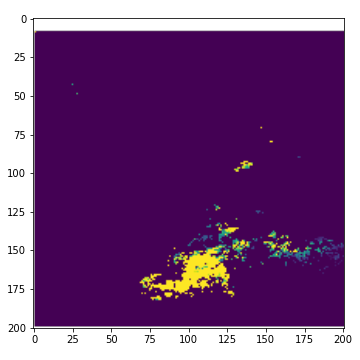
\includegraphics[width=.7\linewidth]{figures/Imagen_CUlia_1.png}
  \caption{\scriptsize Precipitation one day before a landslide}
  \label{fig:culia1}
\end{subfigure}%
\begin{subfigure}{.5\linewidth}
  \centering
  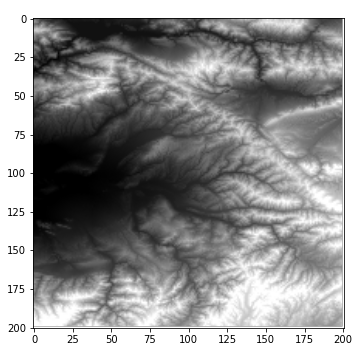
\includegraphics[width=.7\linewidth]{figures/imagen_culia_2.png}
  \caption{\scriptsize Elevation Map shows a region with steep slopes}
  \label{fig:culia2}
\end{subfigure}
\caption{\footnotesize This sample exemplifies how precipitation in a steep region can trigger a landslide event.}
\label{fig:culias}
\end{figure}
% \subsubsection{Data processing}

% \noindent
    
%   From the DEM's maps and by using raster calculators and functions from the software GRASS GIS, it was possible to obtain different layers associated with topographic parameters, for each region of a landslide. These parameters provide additional information to the physical characterization of the terrain. Particularly, in this project it was considered the next five topographical parameters: slope angle, slope aspect, length slope, TWI and SPI, all of them considered as important landslides conditional factors in several previous studies \cite{abedini2019, pourghasemi2013}. A brief description of each factor is provide below:
% \begin{itemize}
%     \item Slope angle: it refers to the mean slope angle of each pixel measured in degrees (°), where an angle of 0° indicates an horizontal terrain and an angle of 90° indicates a fully vertical slope.
%     \item Slope aspect: indicates the orientation with respect of geographical north of the slope of each pixel, measured in degrees. Therefore, a slope aspect of 0° is associated with north and a slope aspect of 180° with south.
%     \item Length Slope (LS): value associated with the length of the slope that passes through each pixel, measured in kilometers. If the terrain is flat, the length slope is taken as 0.03, value approximately equals to the length of the pixel.
%     \item Topographic Wetness Index (TWI): is a topographical index related to the potential of runoff generation of each pixel. This index is calculated by equation (1).
%     \begin{equation}\label{eq:TWI}
%         TWI = \log\left[\frac{a}{\tan(b)}\right]
%     \end{equation}
%     where $a$ is the drainage area upstream of the pixel and $b$ is the slope angle measured in radians. 
%     \item Stream Power Index (SPI): is a topographical index that indicates the erosive potential of a pixel due to the action of water flow. It is calculated by equation (2).
%     \begin{equation}
%         SPI = \log[a \cdot \tan(b)]
%     \end{equation}
%     where $a$ and $b$ are the same variables from equation \eqref{eq:TWI}.
% \end{itemize}
\vspace{5pt}
\subsubsection{Data intersection}
\begin{itemize}
    \item The process starts with the creation of a data structure, from the intersection of the datasets considered in this work (section \ref{ss:datasets-considered}) and Descartes Labs data. From the data extraction, and the data from Descartes Labs, is possible to obtain the SceneCollection dataset. Finally, from this last dataset, attributes such as the number of scenes, the size in megabytes, among others are obtained.

    The plan is to upload this dataset intersection to a new collection or upload this dataset to Google Bucket. Anyway, this section will be more important for the last steps.
\end{itemize}

\subsubsection{Create a Negative Class}\noindent

To create a Negative class, random points were used, with the constraint of being close to the original point from the True class. And selecting random dates which are similar sampled from the True Class. Since the chance of having a landslide using this method is very low, it is accurate  to assume that this method did not add true labeled data points to the negative class.

This points can be seen in the Figure \ref{fig:no-landslide}.

\begin{figure}
  \centering
  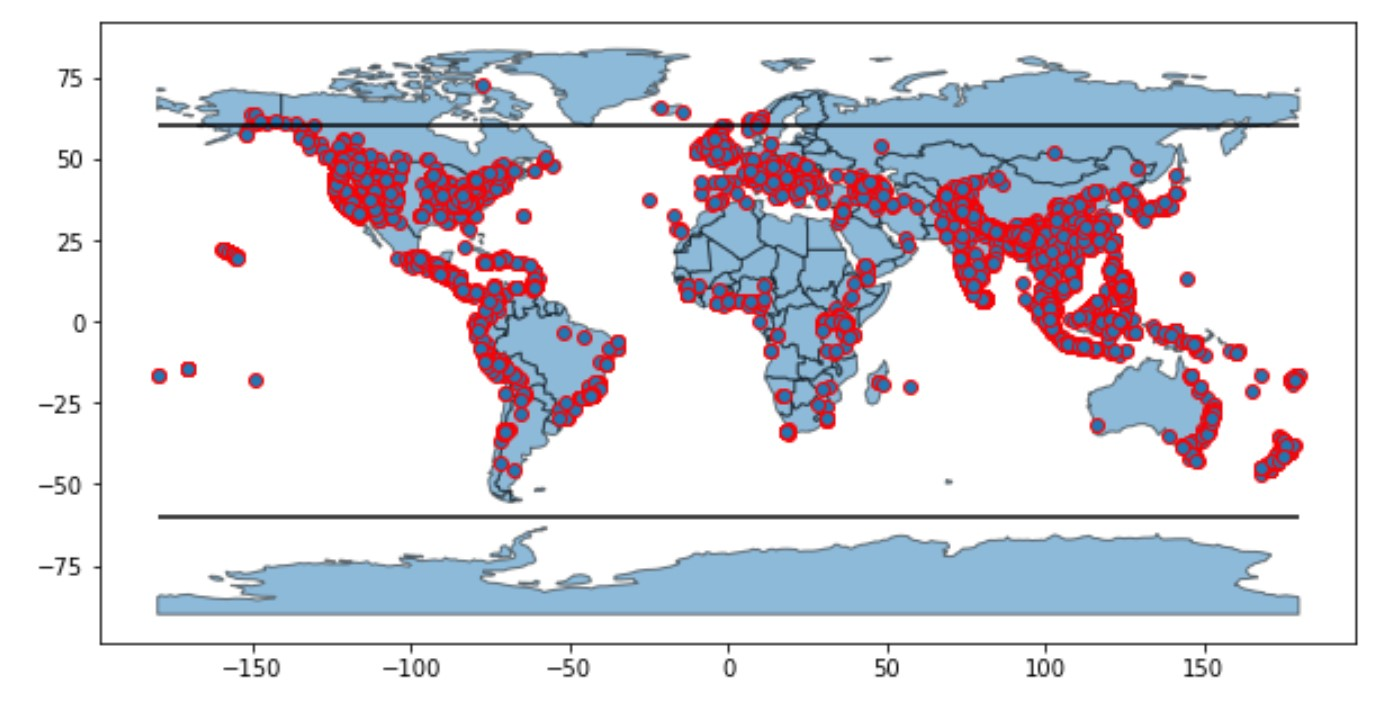
\includegraphics[width=\linewidth]{figures/mapa_no_landslide.jpg}
  \caption{Plot the landslide events in the NASA dataset with the bound longitudes marked as black lines.}
  \label{fig:no-landslide}
\end{figure}
% To create a Negative class, it will use random points, but that were near from an original point from the True class, and selecting random dates which are similar sampled from the True Class. % Para crear la clase negativa, se usaron puntos aleatorios, de forma que estuvieran cerca de los puntos originales de la clase verdadera, y seleccionando fechas aleatorias de forma que estén sampleadas de forma similar a la clase verdadera.

% Una forma alternativa de redactarlo es
% Se ha creado la clase negativa a partir de la clase positiva, de forma que tengan datos similares en geografía y que tenga una distribución de fechas similares.

\subsubsection{Create Training Data} 

\noindent

To create the training data, the values stored in the dataset are extracted and made into a tensor of shape [\textbf{data\_length}, \textbf{n\_t\_frames}, \textbf{n\_channels}, \textbf{width}, \textbf{height}]. With \textbf{data\_length} the number of samples, \textbf{n\_t\_frames} the number of the total time observations, \textbf{n\_channels} the amount of data images stacked on top of each other and the \textbf{width} and \textbf{height} of each image respectively. Then, each stack of images is resized to a fixed \textbf{width} and \textbf{height} and normalized between 0 and 1.

This normalized data is then augmented using image transformations and adding a small noise. Finally the data is separated in a training, validation and test datasets so it is ready to train the model.



\subsection{Landslide Prediction}

For the implementation of the landslide prediction system, the team was highly inspired by implementations of weather nowcasting systems \cite{Forecast_LSTM} that combined a Convolutional Neural Network (CNN) with a LSTM \cite{LSTM} to make weather predictions. %For our objective, the model is composed of a CNN module, that extracts the features for each time measure of the sample wich are feed to aa LSTM that extracts the final features that are 
The proposed model, extracts the features of the 3d data matrix for each time sample using a CNN module adapted for the number of channels. These features are then concatenated to make a sequence that is fed to a LSTM module to extract the sequence features. The final prediction is using a Fully Connected (FC) layer and a sigmoid activation to give the estimated probability of a landslide. 

A diagram of the architecture is illustrated in Figure \ref{fig:CNNLSTM}.%\\

The CNN modules can be interchanged by different CNN architectures. As a first approach, this was designed as a slight modification of ResNet \cite{Resnet} with an added first convolutional layer, an adapted number of input channels and without the final FC layer. This choice was made, because it performs reasonably well in the ImageNet database and there is a builtin implementation of ResNet in Pytorch with several variations of different depths with pretrained weights, so we can use transfer learning to obtain better and faster results. This module can be easily modified to another architecture if there is any need. The LSTM module can also be modified by modifying the number of layers. There is also the opportunity to replace this module with a transformer module \cite{Atention}. 
%The final choice of hyperparameters and the CNN module architecture is still not defined, and it will need several iterations of testing to come to a conclusion.


\begin{figure}
  \centering
  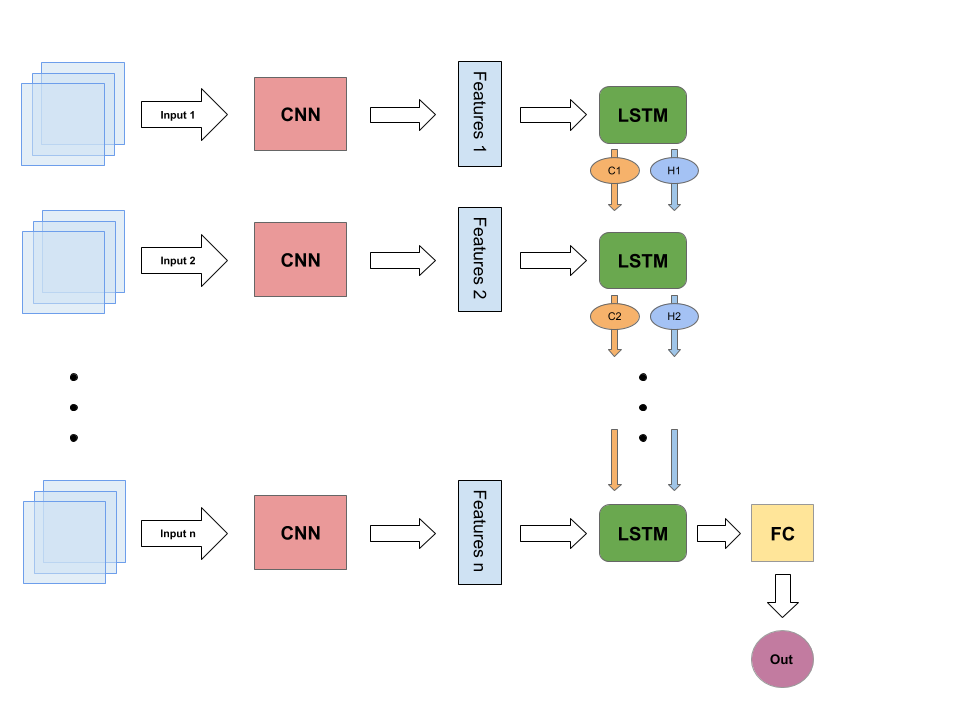
\includegraphics[width=1.2\linewidth]{figures/Architecture CNNLSTM(1).png}
  \caption{General architecture of the implemented CNN LSTM for an input of ``n'' temporal frames. The CNN modules can be interchanged by different architectures.}
  \label{fig:CNNLSTM}
\end{figure}

\subsection{Risk Factor}

To calculate the risk factor of a given disaster is not a trivial matter, %We propose an estimate of this risk by multiplying the estimated probability of a landslide by the logarithm of the addition of the estimated population density with the amount of near road infrastructure. 
an estimated value of this risk is proposed by equation (3).
\begin{equation}
  risk = p \cdot \left( \lambda_0 \ln(P_D) + \lambda_1 R_Z \right)  
\end{equation}

With $p$ the landslide probability estimated by the landslide predictor, $P_D$ the estimated population density near the disaster, $R_Z$ the amount of nearby road zones and $\lambda_0, \lambda_1$ some positive weights to adjust the relevance of each component.

Even so, it is still difficult to know exactly the population density and the amount of nearby roads. A good guess for the population density would be the amount of people living nearby according to the national census. For the road zones, a proposed solution could be the total sum of the binarized road map of the zone.

This approaches still rely on scarce and unreliable data given government offices, especially on developing countries. %But this approach could be feasible for the ProjectX competition.

Unfortunately, due to limitations of the access to this data, experiments of the risk factor had to be postponed and instead will be considered as future work.

%\subsection{Outline of the Methodology}
%\lipsum[1]

\section{Experiments and Results}

% Resultados de datasets
% Resultados de ocupar los datasets en el modelo
% Próximos pasos // Esto va en la otra seccion

% Datos importantes
% Tamaño del Dataset CHIRPS, CFS y GSOD fue de un total de 500 GB,
% Cada Batch de tamaño 160 pesaba 4.7 GB
% Modus Operandis:
% Primero se extrajo información de los satélites por medio de la API de DescartesLab
% Se almacena la información de los 3 satélites en archivos .npy, ordenado por fechas

% Generación de Dataset para el Modelo
% 1.- Se intersectan las fechas de los 3 satélites, para así obtener datos donde los 3 satélites hayan hecho mediciones en un día específico
% 2.- Se ordenan los días para que vayan desde la fecha más alejada, a la más actual
% 3.- Se crea un tensor con 160 datos de cada satélite, este tensor es de la forma (datos, dias, canales, ancho, alto) donde datos son la cantidad de datos del satélite, en este caso 160 datos por cada tensor, los días son los datos de días anteriores, en este caso todos los satélites cuenta sus datos, y datos de 9 días hacia atras.
% 4.- Se Mergean los datos, tomando cada batch de 160 de cada satélite, y juntándolos en un solo tensor con la suma de sus canales (teniendo la precaución que el batch que se tome corresponde al mismo día)

% De esta forma se arma un sandwich para que la red se la coma. 

% Complicaciones
% El tamaño del sandwich es extremadamente grande como para que la red lo pueda procesar correctamente, un sandwitch es del orden de 4.31 GiB, teniendo en cuenta que son 50 + 37 partes en total, esto da un dataset del tamaño de 375 GiB

% Se decide particionar los datos en batch de tamaño 5, sin solución.

% Se opta por entrenar la red solo con los datos de CHIRPS, para evaluar efectividad de la red.


\begin{table}
\caption{Data sizes of each satellite products.}%estimated data size}
\begin{tabular}{|c|c|}
\hline
\textbf{Satellite} & \textbf{Size {[}GiB{]}} \\ \hline
CFS                & 234.6                   \\ \hline
CHIRPS             & 23.46                   \\ \hline
GSOD               & 205,9                   \\ \hline
Total Sum          & 463,96                  \\ \hline
\end{tabular}
\end{table}

The landslide prediction model was also tested on a toy dataset to verify the expected inner workings of the model and training loop.

The first experiments where done with the training of the landslide prediction model over the whole dataset of satellites. Unfortunately, due to the size of all this data 

The first version of the model was trained with precipitation data coming from the CHIRPS satellite. Here, the model achieved an accuracy of $77\%$ in the training data with a similar accuracy on the validation data. This result can be observed on Figure \ref{fig:resultado01}. 


 \begin{figure}
  \centering
  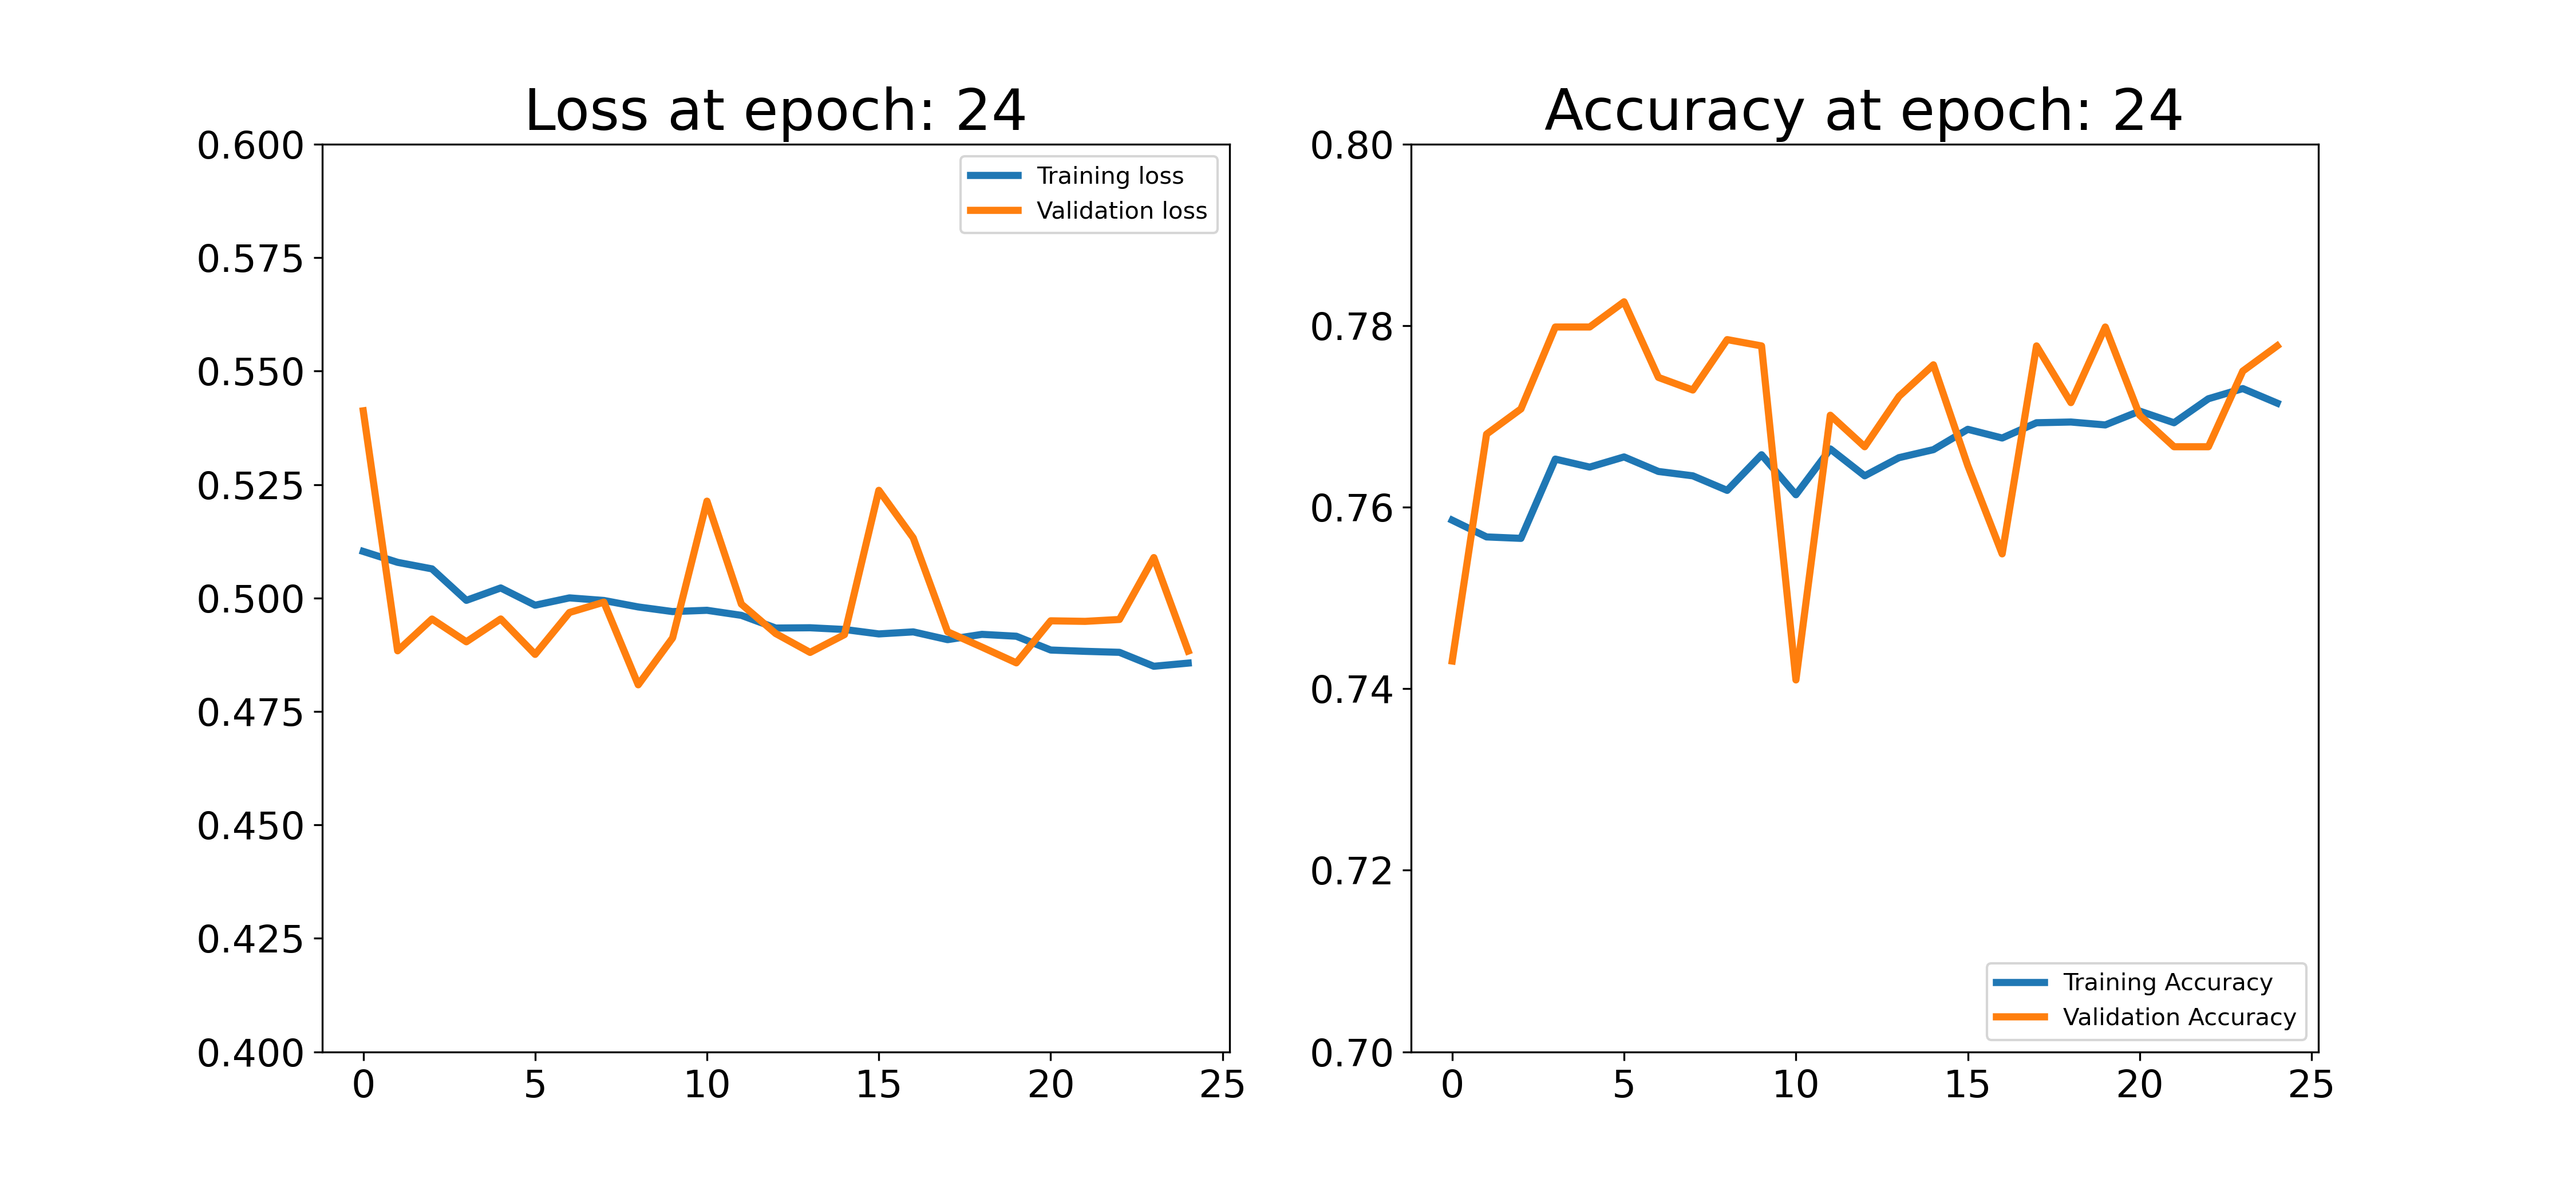
\includegraphics[width=1.1\linewidth]{figures/the_final.png}
  \caption{Loss and accuracy with CHIRPS data.}
  \label{fig:resultado01}
\end{figure}

%The next steps in the project are:
%\begin{itemize}
 %   \item To create an unified dataset with the recollected data.
  %  \item To perform a Exploratory Data Analysis.
   % \item To obtain false cases for landslide detections and label the data.
    %\item To train the model on the dataset.
%    \item To tune the hyperparameters of the model by testing.
 %   \item To estimate the risk for a landslide on the test data.
  %  \item To draw conclusions and observations.
%\end{itemize}


\section{Discussion}
\subsection{Analysis of Results and Methods}

From the Figure \ref{fig:resultado01}, it can be observed how the landslide model gives a reasonable prediction even at the early epochs and using data from a single source. This results allow to establish a minimum expected performance of the model, and by adding the remaining satellites and increasing the model depth, the results should improve. Considering that the accuracy of the model is already over $75\%$, a similar landslide prediction model using ML shows promise for real life applications. 

\subsection{Applicability}

The main purpose of this model is to help emergency services to allocate resources more efficiently and avoid the potential loss of human life. 

\section{Limitations and future work}

Firstly, the intention was to apply the model built in Continental Chile, but by several limitations in the availability and access of essential information (e.g. georeferenced location of historical landslides in the country and precipitation data in real time) the original approach had to change. For this reason, the model was trained only with data from satellites and the area of application was expanded to be used in any location in the world.

% Dejar la red un tiempo infinito a futuro, pues ahora lo corrimos en muy pocas épocas 
Defined the final approach of this work, the biggest limitation experienced during the experiments was produced by the data transfer rate for loading the data of all the satellites, reaching the extreme that some of the tensors took between 30 to 40 seconds to load. Therefore, training the CNN LSTM network in a reasonable time was not feasible. 

There was also the limitation of area covered by the satellites since not all the planet is covered. In figure \ref{fig:no-landslide} we can see the limitation of the longitudes for one of the satellites, this implied that some data points had to be discarded from the dataset.

% Iterar el modelo o quizás obtener otras features de data que no estamos considerando
For future work, a logical extension might be to use all the satellite data gathered or even include more sources. The reason for not using more data was due to the time restrains of the ProjectX competition and the processing time of the database. 

Some other work that could be studied in the future is the differences in the performance with different layer depths and replacing the LSTM block with Attention. 

% Ocupar el risk factor en un trabajo futuro
Another component that originally was intended to be in the work was a risk factor which was dependent of the urbanization levels. The risk calculation would be useful in particular for governmental organizations that seek to alert the population early in order to save life's under landslide risk.

% Hacer una regularización entrenando múltiples modelos


\section{Conclusion}
%  I enjoy to work with you guys <3 <3 <3

The present work explored the viability of the use of machine learning models for landslides early warning prediction. This opens a wide range of applications, such as early evacuation programs for vulnerable areas, urban planning and strengthen the monitoring networks in developed countries. All in all, the use of this kind of models can improve the resilience of both decision-making and communities.

In this project was proposed a general architecture that involves a two block model. On one hand, a two-dimensional convolutional layers was used to retrieve important spatial features. This block is expected to use all the information provided by the different bands in order to obtain both weather and topographical understanding. The resulting features were fed to a LSTM in order to give the causal nature of the data for a sequence of days. Finally, a fully connected layer was used to interpret this as a probability of the event happening.


%\section{Proposed Solutions/Methods}

%At this point of the research process, we have the following proposed solutions to answer the question: %

%\begin{enumerate}
%    \item Combination of LSTM and Convolutional Networks.
%    \item MOGPS with spectral mixture.
%\end{enumerate}

%The idea behind implementing  LSTM and Convolutional networks is to be able to combine both satellite and geographic data on a time series fashion.  

%The implementation of MOGPS's offers an extremely powerful tool to work with time series, even detecting small correlations between several sources, allowing it to make accurate future predictions in complex systems. 

%The human risk factor has to be considered in the implementation, due to the limited resources that emergency rescue organizations operate, its important to prioritize response to critical areas. 





%\section{Workflow}

%At this time, the estimated workflow is as follows for the next two and a half months: 

%\begin{enumerate}
%    \item Data pre-processing, cleanup and visualization (2 weeks).
%    \item Preparation of work environment (1 week).
%    \item Testing viability of models and definition of final implementation(1 week). 
%    \item Training (3 weeks).
%    \item Results analysis (1 week).
%    \item Paper redaction (2 weeks).
%\end{enumerate}


\bibliographystyle{ACM-Reference-Format}
\bibliography{sample}

\end{document}
\endinput
